\subsection{Stability}
\label{sec:dcqcn_stability}

\begin{figure*}[t]
\center
\subfigure[Default parameters ($R_{AI}=40Mbps$, $K_{max}=200KB$).]
{
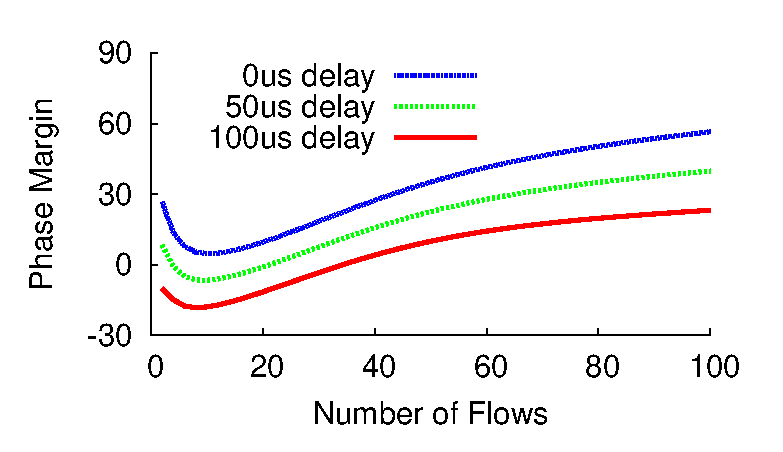
\includegraphics[width=0.3\textwidth]{figures/dcqcn_stability.eps}
\label{fig:dcqcn_stability_default}
}
\subfigure[$R_{AI}=10Mbps$.]
{
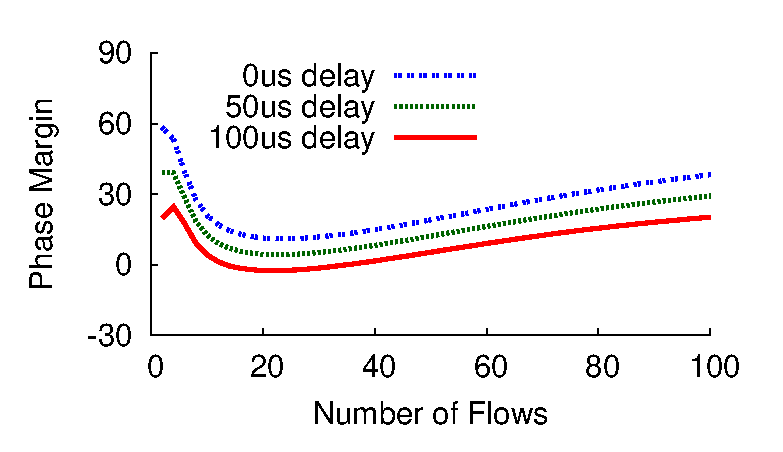
\includegraphics[width=0.3\textwidth]{figures/dcqcn_stability_rai.eps}
\label{fig:dcqcn_stability_rai}
}
\subfigure[$R_{AI}=10Mbps$ and $K_{max}=1000KB$.]
{
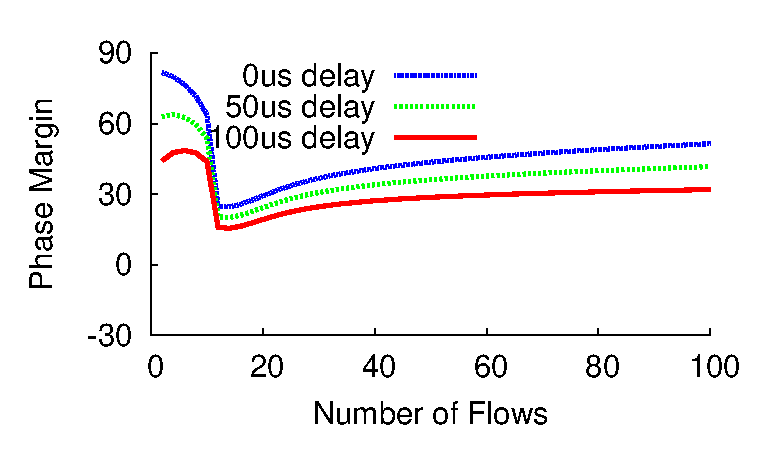
\includegraphics[width=0.3\textwidth]{figures/dcqcn_stability_rai_kmax.eps}
\label{fig:dcqcn_stability_rai_kmax}
}
\caption{DCQCN stability}
\label{fig:dcqcn_stability}
\end{figure*}
To analyze stability, we first obtain the fixed point of the system, and then
linearize the model around the fixed point. We analyze the linearized model for
stability using classical frequency domain techniques~\cite{controltheory}.  

\begin{thm}[DCQCN's unique fixed point]
A unique fixed point exists for DCQCN. At this fixed point, all flows converge to the same rate. 
\end{thm}
\begin{proof}
By setting the left-hand side of Equation~\ref{eq:q} to 0,
it is easy to see that any fixed points of the DCQCN (if they exist) must
satisfy:
\begin{equation}
\small
\sum\limits_{i = 1}^N {R_C^{(i)}(t)} = C
\label{eq:fixedrc}
\end{equation}
At any of the fixed points, we assume the value of $p$ is $p^*$, which is shared
by all flows. The queue length and per-flow $\alpha^{(i)}$ at the fixed points
are determined by Equation~\ref{eq:mark} and \ref{eq:alpha}:
\begin{equation}
\small
{q^*} = \frac{{{p^*}}}{{{p_{max}}}}\left( {{K_{max}} - {K_{min}}} \right) + {K_{min}}
\end{equation}
\begin{equation}
\small
\alpha^{(i)*}  = 1 - {(1 - p^*)^{{\tau '}R_C^{(i)*}}}
\end{equation}
Next, we show that $p^*$ exists and is uniquely determined by $R_C^{(i)*}$ in
the DCQCN model.  From Equation~\ref{eq:rt} and \ref{eq:rc}, at the fixed point,
we get the two forms of $R_T^{(i)*}$, respectively:
\begin{equation}
\small
{R_T^{(i)*}} = R_C^{(i)*} + \frac{{a\alpha^{(i)*} }}{{(b + d)\tau }}
\end{equation}
\begin{equation}
\small
{R_T^{(i)*}} = R_C^{(i)*}\left( {1 + \frac{{(c + e)\tau {R_{AI}}}}{a}} \right)
\end{equation}
Where we denote $a, b, c, d, e$ as follows:
\begin{equation}
\small
\begin{array}{l}
a = 1 - {(1 - p^*)^{\tau {R_C^{(i)*}}}},b = \frac{{p^*}}{{{{(1 - p^*)}^{ - B}} - 1}},c = \frac{{{{(1 - p^*)}^{FB}}p^*}}{{{{(1 - p^*)}^{ - B}} - 1}},\\
d = \frac{{p^*}}{{{{(1 - p^*)}^{ - T{R_C^{(i)*}}}} - 1}},e = \frac{{{{(1 - p^*)}^{FT{R_C^{(i)*}}}}p^*}}{{{{(1 - p^*)}^{ - T{R_C^{(i)*}}}} - 1}}
\end{array}
\end{equation}
Combining the two forms of $R_T^{(i)*}$, we see that the value of $p^*$ is determined by:
\begin{equation}
\small
\frac{{{a^2}\alpha^{(i)*} }}{{(b + d)(c + e)}} = {\tau ^2}{R_{AI}}R_C^{(i)*}
\label{eq:p_fixed}
\end{equation}
The LHS of Equation (\ref{eq:p_fixed}) is monotonic when $p \in [0,1]$.
Furthermore, when $p = 0$, the LHS is smaller than RHS, and vice versa when $p =
1$. Thus DCQCN has a unique fixed point, determined by a unique $p^*$.
Numerical analysis shows that $p^*$ is typically very close to 0.  Therefore, we
approximate the LHS using Taylor series around $p=0$:
\begin{equation}
\small
\frac{{{a^2}\alpha }}{{(b + d)(c + e)}} = \frac{{(R_C^{(i)*})^3{\tau ^2}\tau '}}{{{{\left( {\frac{1}{B} + \frac{1}{{TR_C^{(i)*}}}} \right)}^2}}}{p^3} + O\left( {{p^4}} \right)
\end{equation}
Omitting the $O(p^4)$ term, and combining with Equation~\ref{eq:p_fixed}, we have the fixed point of $p$:
\begin{equation}
\small
{p^*} = \sqrt[3]{{\frac{{{R_{AI}}}}{{{\tau '}(R_C^{(i)*})^2}}{{\left( {\frac{1}{B} + \frac{1}{TR_C^{(i)*}}} \right)}^2}}}
\label{eq:fixedp}
\end{equation}
From the equation above, we see that $p^*$ and $R_C^{(i)*}$ uniquely determine each other. 
Since $p^*$ is shared by all flows $i$, $i = 1, 2, ..., N$, we have:
\begin{equation}
\small
R_C^{(1)*} = R_C^{(2)*} = ... = R_C^{(N)*}
\end{equation}
Combining this with Equation~\ref{eq:fixedrc}, proves that there is only one
unique fixed point, at which $R_C^{(i)*} = \frac{C}{N}$, $i = 1, 2, ..., N$ and
$p^*$ is given by Equation~\ref{eq:fixedp}.
\end{proof}

\para{Stability analysis.} 
We linearize the system by denoting $\delta {R_C}(t) = {R_C}(t) - R_C^*$,
$\delta {R_C}(t) = {R_C}(t) - R_C^*$, $\delta p(t) = p(t) - p^*$, $\delta \alpha
(t) = \alpha (t) - \alpha^*$, and $A = \left( {\frac{1}{B} + \frac{1}{{TR_C^*}}}
\right)$.  We again use Taylor series to simplify the expressions of $a, b, c,
d, e$ to handle the exponential forms like $(1-p)^x$.  Due to lack of space,
here we only just show the linearized expression for $\frac{{d\delta {R_C}}}{{dt}}$:
\begin{equation}
\small
\begin{array}{l}
\frac{{d\delta {R_C}}}{{dt}} =  - \frac{1}{2}{(R_C^*)^2}{\alpha ^*}\delta p - \frac{1}{2}{p^*}R_C^*{\alpha ^*}\delta R_C \\
 - \frac{1}{2}{p^*}R_C^*{\alpha ^*}\delta {R_C} - \frac{1}{2}{p^*}{(R_C^*)^2}\delta \alpha \\
 + \frac{A}{2}\left( {R_C^*\delta {R_T} - R_C^*\delta {R_C} + R_T^*\delta {R_C} - R_C^*\delta R_C} \right)\\
 - \left( {\frac{1}{2} + \frac{A}{4}} \right)\left( {{p^*}R_C^*\delta {R_T} - {p^*}R_C^*\delta {R_C} + {p^*}R_T^*\delta {R_C}} \right)\\ 
 - \left( {\frac{1}{2} + \frac{A}{4}} \right)\left( {{p^*}R_C^*\delta R_C - R_C^*R_T^*\delta p + {{(R_C^*)}^2}\delta p} \right)
\end{array}
\end{equation}
Using Laplace transform, we get:
\begin{equation}
\small
\begin{array}{l}
s{R_C}(s) - \delta {R_C}(0) = \\
\left( { - \frac{1}{2}{{(R_C^*)}^2}{\alpha ^*} - \left( {\frac{1}{2} + \frac{A}{4}} \right)R_C^*R_T^* + \left( {\frac{1}{2} + \frac{A}{4}} \right){{(R_C^*)}^2}} \right){e^{ - s\tau *}}p(s)\\
 + \left( { - \frac{1}{2}{p^*}R_C^*{\alpha ^*} - \frac{A}{2}R_C^* + \left( {\frac{1}{2} + \frac{A}{4}} \right){p^*}R_C^*} \right){e^{ - s\tau *}}{R_C}(s)\\
 + \left( { - \frac{1}{2}{p^*}R_C^*{\alpha ^*} - \frac{A}{2}R_C^* + \frac{A}{2}R_T^* }\right){R_C}(s)\\
 + \left( { \left( {\frac{1}{2} + \frac{A}{4}} \right){p^*}R_C^* - \left( {\frac{1}{2} + \frac{A}{4}} \right){p^*}R_T^*} \right){R_C}(s)\\
 - \frac{1}{2}{p^*}{(R_C^*)^2}\alpha (s)\\
 + \left( {\frac{A}{2}R_C^* - \left( {\frac{1}{2} + \frac{A}{4}} \right){p^*}R_C^*} \right){R_T}(s)
\end{array}
\end{equation}
With Laplace transform of the other equations, we can use ${R_C}(s)$ to express
${R_T}(s)$, $p(s)$ and $\alpha (s)$.  We then derive the characteristic equation
of ${R_C}(s)$. We test the characteristic equation against {\em Bode Stability
Criteria}~\cite{controltheory}. The results are shown in
Figure~\ref{fig:dcqcn_stability}.  The degree of stability is shown as {\em
Phase Margin}. The system is stable when its {\em Phase Margin} is larger than
0, and the larger {\em Phase Margin} means the system is more stable.

We analyze DCQCN stability in different conditions, particularly with different
control signal delays (propagation delay plus queuing delay in practice), and
different number of flows. An ideal protocol should be tolerant with large delay
and scalable to any number of flows. As Figure~\ref{fig:dcqcn_stability} shows,
DCQCN, with default parameters, is mostly stable. In most cases, the phase
margin is larger than 0.
\begin{figure}[t]
\subfigure[] {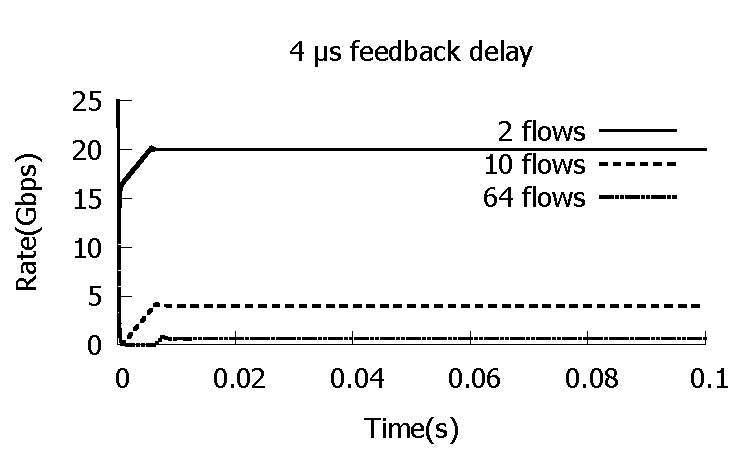
\includegraphics[width=0.49\columnwidth]{figures/stable_rate_4.pdf}}
\subfigure[] {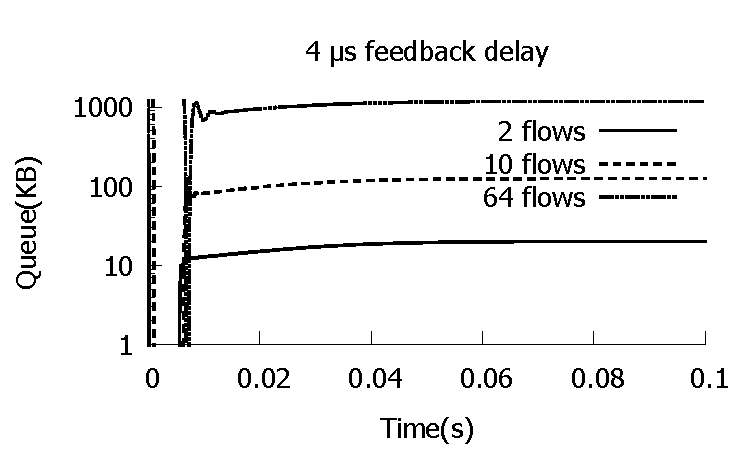
\includegraphics[width=0.49\columnwidth]{figures/stable_q_4.pdf}}
\subfigure[] {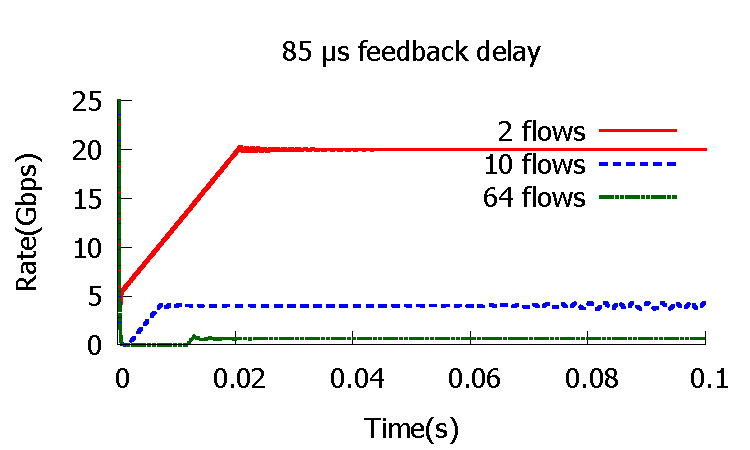
\includegraphics[width=0.49\columnwidth]{figures/stable_rate_85.pdf}}
\subfigure[] {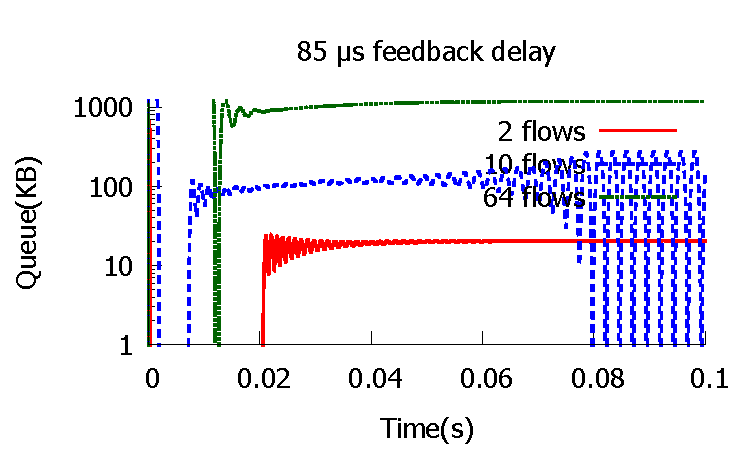
\includegraphics[width=0.49\columnwidth]{figures/stable_q_85.pdf}}
\caption{Impact of delay and number of flows on DCQCN stability}
\label{fig:dcqcn_unstable}
\end{figure}



\begin{figure*}[t]
\centering
\mbox{
\begin{minipage}{0.31\textwidth}
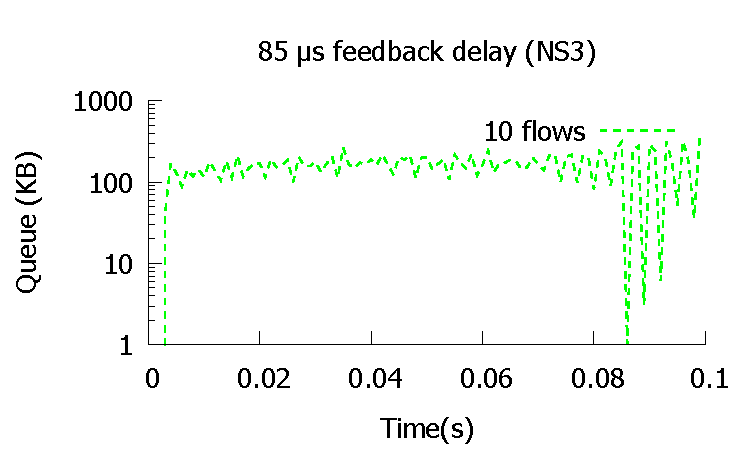
\includegraphics[width=0.99\columnwidth]{figures/stable_queue_85_ns.pdf}
\vspace{-1em}
\caption{NS simulations confirm lack of stability}
\vspace{-1em}
\label{fig:dcqcn_unstable_ns}
\end{minipage}
\hspace{0.02in}

\begin{minipage}{0.37\textwidth}
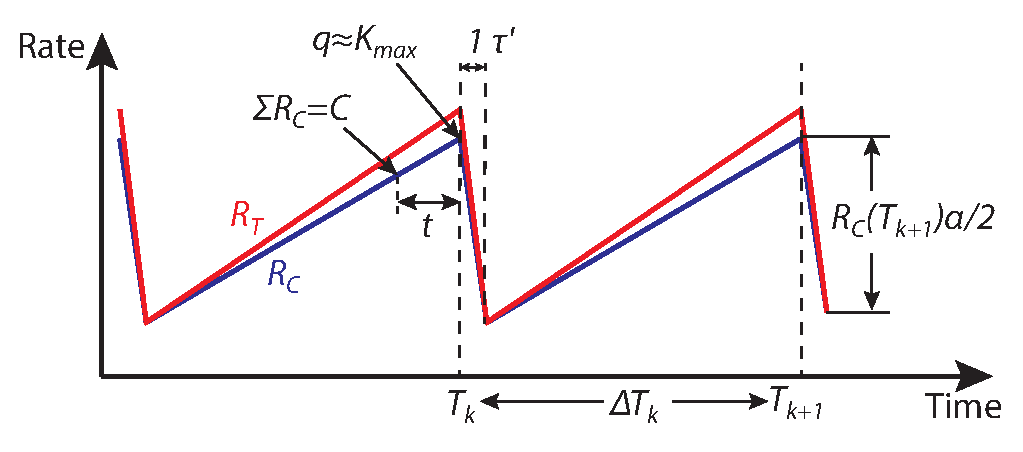
\includegraphics[width=0.99\columnwidth]{figures/dcqcn_convergence.eps}
\vspace{-1em}
\caption{DCQCN flow rate update.}
\vspace{-1em}
\label{fig:dcqcn_convergence}
\end{minipage}
\hspace{0.02in}

\begin{minipage}{0.31\textwidth}
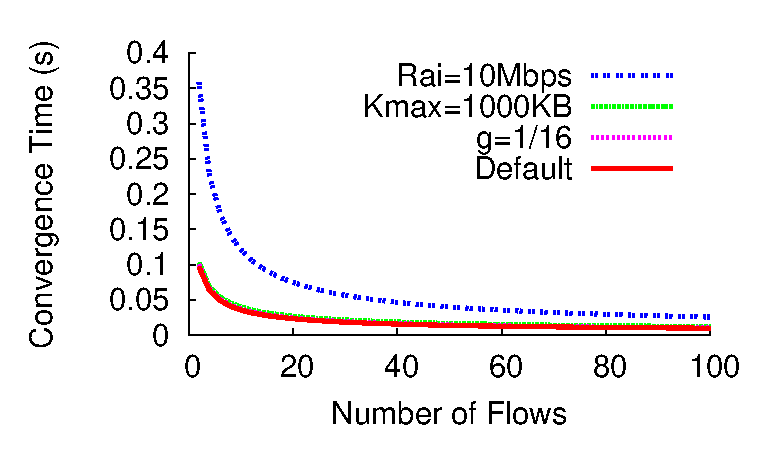
\includegraphics[width=0.99\columnwidth]{figures/dcqcn_convergence_time.eps}
\vspace{-1em}
\caption{Upper bound on DCQCN convergence time under conservative assumptions}
\vspace{-1em}
\label{fig:dcqcn_convergence_time}
\end{minipage}
}
\end{figure*}

%\begin{figure}[t]
%\center
%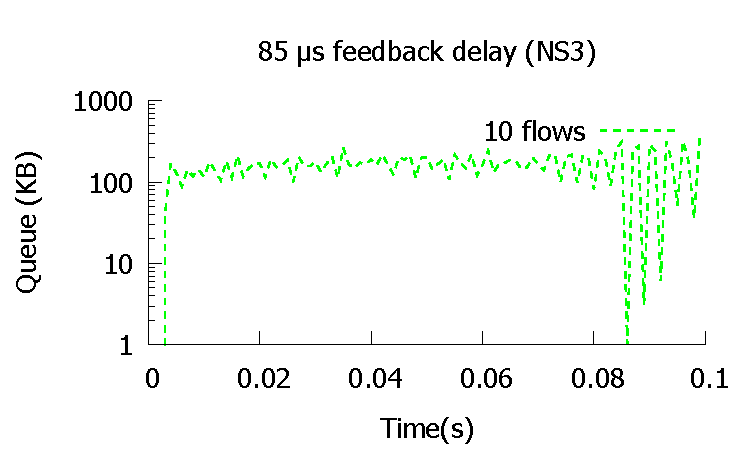
\includegraphics[width=0.4\textwidth]{figures/stable_queue_85_ns.pdf}
%\caption{NS simulations confirm lack of stability}
%\label{fig:dcqcn_unstable_ns}
%\end{figure}

Curiously, unlike TCP, the relationship between number of flows and the phase
margin is non-monotonic. When the delay is large, {\em e.g., 100$\mu$s}, the
phase margin dips below zero for certain number of flows, before rising again.
For the set of parameters we have chosen, the system can be unstable with 10
flows at high feedback delays.  DCQCN is increasingly stable with larger number
of flows, which means good scalability. This point is further illustrated in the
fluid model results shown Figure~\ref{fig:dcqcn_unstable}. When the feedback
delay is small (4 $\mu$s), DCQCN is stable - flow rates, and queue length
quickly\footnote{Remember that DCQCN flows always start at line rate.}
stabilizes regardless of the number of flows. However, when the delay is large
(85$\mu$s), the protocol is unstable for 10 flows. It is, however, stable for 2
and 64 flows. Figure~\ref{fig:dcqcn_unstable_ns} confirms that we observe the
same instability in packet-level simulations.

While this problem may not be particularly serious in practice, it can be easily 
fixed by tuning the values of $R_{AI}$ and $K_{max}$.  Smaller $R_{AI}$
means flows increase their rate more gently, and stabilizes the system.
Similarly, larger $K_{max} - K_{min}$ makes rate decreasing more fine grained,
because the perturbation of queue length leads to smaller marking probability
perturbation. We show these trends in Figures \ref{fig:dcqcn_stability_rai} and
\ref{fig:dcqcn_stability_rai_kmax}.  With small $R_{AI}$ and large $K_{max}$,
DCQCN can be always stable even when the control signal delay reaches 100$\mu
s$, which equals to the propagation delay of a $30KM$ cable, or $500KB$ queuing
delay. Such large delays are rare in modern datacenter networks. 

Note that tuning $R_{AI}$ and $K_{max}$ is a trade-off between stability and
latency. Smaller $R_{AI}$ leads to slower ramp-up, while larger $K_{max}$ leads
to larger queue length. In most cases, the default parameters strike a good
enough balance between stability and latency.
